\documentclass[11pt,a4paper]{article}
\usepackage[utf8]{inputenc}
\usepackage{amsmath}
\usepackage{amsfonts}
\usepackage{amssymb}
\usepackage{parskip}
\usepackage{tikz}
\usepackage[margin=1in]{geometry}
\usepackage{graphicx}
\usetikzlibrary{arrows,positioning} 
\tikzset{
    %Define standard arrow tip
    >=stealth',
    %Define style for boxes
    punkt/.style={
           circle,
           rounded corners,
           draw=black, very thick,
           text width=2.5em,
           minimum height=2em,
           text centered},
    % Define arrow style
    pil/.style={
           ->,
           thick,
           shorten <=2pt,
           shorten >=2pt,}
}


\author{Finnian Lattimore}
\title{A short introduction to causal inference}

\begin{document}
\def\ci{\perp\!\!\!\perp} % from Wikipedia

\section{Why is causality important}

\section{Models of causality}
To understand causality we first need a more formal definition of what we are talking about. In this post we will look at three slightly different definitions of causality and use them to describe the following very simple example. This section aims to demonstrate the notations and formalisms we will need to tackle more interesting problems later on.

We have developed a new drug for some illness and wish to determine how effective it is. We take a large group of patients and randomly assign half of them to a treatment group and the other half to a control group. The people in the treatment group get the drug, everyone else gets a placebo pill. The question we want to answer is does giving people the active drug improve their changes of recovery relative to giving them the placebo. We will use the variable $X$ (1 = drug, 0 = placebo) to represent the treatment each person receives and $Y$ (1 = recover, 0 = not recover) to describe the outcome .
\subsection{Structural Equation Models}

Structural equation models (SEMs) describe a deterministic world, where underlying mechanisms determine the output of any process for a given input. The mechanism (but not the output) is assumed to be independent of what is fed into it. Linear structural equation models have a long history for causal estimation \cite {Wright1921,Haavelmo1943}. More recently, they have been formalized, generalized to the non-parametric setting and connected to developments in graphical models to provide a powerful causal framework \cite{Pearl2000}.

Mathematically, each variable is a deterministic function of its direct causes and a noise term that captures unmeasured variables. The noise terms are required to be mutually independent. If there is the possibility that an unmeasured variable influences more than one variable of interest in a study, it must be modelled explicitly as a latent (unobserved) variable. Structural equation models can be represented visually as a network. Each variable is a node and arrows are drawn from causes to their effects. For our example the SEM is:

\[
\begin {aligned}
X = & \epsilon_{x} \\
Y = & f(X,\epsilon_{y})
\end {aligned}
\qquad
\raisebox{-5mm}
{
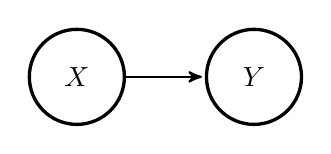
\begin{tikzpicture}[->,>=stealth',shorten >=1pt,auto,node distance=1cm,
  thick,main node/.style={punkt}]

 %nodes
\node[main node](1){$X$};
\node[main node, right=of 1](2){$Y$};


 \path[every node/.style={font=\sffamily\small}]
    (1) edge node {} (2);
	
\end{tikzpicture}
}
\]

This model encodes the assumption that the outcome $y_{i}$ for an individual $i$ is caused solely by the treatment $x_{i}$ they receive and other factors $\epsilon_{y_{i}}$ that are independent of $X$. This is justifiable on the grounds that $X$ is random; the outcome of a coin flip for each patient should not be related to any of their characteristics (hidden or otherwise). 

We want to estimate the causal effect of treatment; what is the probability of recovery if we \textbf{take the action} 'treat' versus the \textbf{action} 'placebo'? 



CONSIDER SOLVING THIS JUST FROM THE FUNCTIONAL POINT OF VIEW. MOVE THE DO NOTATION DOWN TO CAUSAL BAYES NETS.




For a model with $N$ variables, a structural equation model looks like a set of $N$ simultaneous equations, with each variable playing the role of the dependent (left hand side) variable in one equation. However a SEM is, by definition, more than a set of simultaneous equations. By declaring it to be structural we are saying that it represents assumptions about the relationships between variables. When we visualise the model as a network the absence of an arrow between two variables encodes the assumption that one does not cause the other.

\subsection{Causal Bayesian Networks}
Causal Bayesian Networks are, unsurprisingly, an extension of Bayesian Networks. Any joint probability distribution can be factorized into a product of conditional probabilities. There are multiple valid factorizations, corresponding to permutations of variable ordering.

\begin{equation}
P(X_{1},X_{2},X_{3},...)=P(X_{1})P(X_{2}|X_{1})P(X_{3}|X_{1},X_{2})...
\end{equation}

We can represent this graphically by drawing a network with a node for each variable and adding links from the variables on the right hand side to the variable on the left for each conditional probability distribution (figure~\ref{fig:bayesnet}). If there are conditional independencies between variables the factorization simplifies, which is reflected by missing edges in the corresponding network. 

\begin{figure}[h]
\centering
\caption{General Bayesian Network over 3 variables}
\label{fig:bayesnet}
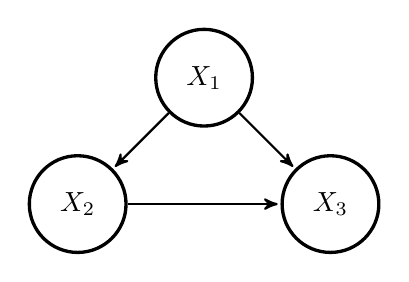
\begin{tikzpicture}[->,>=stealth',shorten >=1pt,auto,node distance=1cm,
  thick,main node/.style={punkt}]

 %nodes
\node[main node](1){$X_{1}$};
\node[main node, below left=of 1](2){$X_{2}$};
\node[main node, below right=of 1](3){$X_{3}$};


 \path[every node/.style={font=\sffamily\small}]
    (1) edge node {} (2)
    	edge node {} (3)
    (2) edge node {} (3);
	
\end{tikzpicture}
\end{figure}

The statement that a given graph $G$ is a Bayesian network for a distribution $P$ tells us that the distribution can be factorized over the nodes and edges in the graph. There can be no missing edges in $G$ that do not correspond to conditional independencies in $P$ (the converse is not true $G$ can have extra edges). If we let $parents_{X_{i}}$ represent the set of variables that are parents of the variable $X_{i}$ in $G$ then we can write the joint distribution as; 

\begin{equation}
P(X_{1}...X_{N}) = \prod_{i = 1...N}P(X_{i}|parents_{X_{i}})
\end{equation}

A CBN is a Bayesian network in which it a link $X_{i} \rightarrow X_{j}$, by definition, implies $X_{i}$ causes $X_{j}$. This means that if we intervene and change the value of $X_{i}$, we expect $X_{j}$ to change, but if we intervene to change $X_{j}$, $X_{i}$ will not change. More generally, if $G$ is a causal network for a distribution $P$ defined over variables $X_{1}...X_{N}$, then we can calculate the distribution after an intervention where we set $Z \subset X$ to $z$, denoted $do(Z=z)$ by simply dropping the terms for each of the variables in $Z$ from the factorization given by the network \cite{Pearl2000}.

\[
 P_{do(Z=z)}(X_{1}...X_{N}) =
  \begin{cases}
  \prod_{i \notin Z}P(X_{i}|parents_{X_{i}}) & \text{$X_{1}...X_{N}$ consistant with $Z=z$}  \\
   0       & \text{otherwise } 
  \end{cases}
\]


Causal Bayesian networks encode information on all interventional distributions over a set of variables. A causal network represents (much) more information than a Bayesian network with identical structure due to the assumption that links can be interpreted causally. Causal Bayesian networks are Bayesian networks so results that apply to Bayesian networks carry directly across;the local markov property states that variables are independent of their non-effects given their direct causes. Similarly the global markov property and d-separation also hold in causal networks. There is an algorithm \cite{Shpitser2012} based on these properties that, for a given network and interventional (do-type) query, can:

a) determine if the query can be translated into an expression involving only distributions over observed variables. In other words, determine if the query is identifiable given the assumptions encoded by the network

b) if it is identiable, return the required expression



Returning at last to our simple example, and phrasing our query in terms of interventions; what would the distribution of outcomes look like if everyone was treated $P(Y|do(X=1))$, relative to if no one was treated $P(Y|do(X=0))$? 

assume the network has the same form as 



We have adopted the do-notation, \cite{Pearl1995}, to distinguish the act of intervening to force X to a given value, from observing it to be that value. In our simple example $P(Y|do(X)) = P(Y|X)$. More generally, for a given SEM and interventional query, there is an algorithm  that can:



\subsection{Counterfactuals and the Neyman-Rubin framework}

The Neyman-Rubin model \cite{Rubin1974,Rubin1978,Rosenbaum1983, Rubin2005,Rubin2008} defines causality in terms of potential outcomes, or counterfactuals. Counterfactuals are statements about imagined or alternate realities, are prevalent in everyday language and may play a role in the development of causal reasoning in humans \cite{Weisberg2013}. Causal effects are differences in counterfactual variables; what is the difference between what would happen if we did one thing versus what would happen if we did something else. 

In our example, the causal effect of the drug relative to placebo for person $i$ is the difference between what would happen if they were given the drug, denoted $y_{i}^{1}$ versus what would happen if they got the placebo, $y_{i}^{0}$. The fundamental problem of causal inference is that we can only observe one of these two outcomes, since a given person can only be treated or not treated. The problem can be resolved if, instead of people, you have units you can assume are identical or that will revert exactly to their initial state some time after treatment. This type of assumption often holds to a good approximation in the natural sciences and explains why researchers in these fields are less concerned with causal theory. 

Instead of trying to estimate individual effects, lets see if we can learn something about the distributions under treatment or placebo.  Let $Y^{1}$ be a random variable representing the potential outcome if treated. The distribution of $Y^{1}$ is the distribution we would see of $Y$ if everyone was treated. Similarly $Y^{0}$ represents the potential outcome for the placebo. We want to know the difference between the probability of recovery, across the population if everyone was treated, and the probability of recovery given placebo  $P(Y^{1})-P(Y^{0})$. We can estimate, from an experimental or observational study, the probability that people recover if treated $P(Y|X=1)$ and the probability that they recover if not treated $P(Y|X=0)$. Now if $X=0$ then $Y = Y^{0}$. Equivalently stated:

\begin{equation}
\begin{aligned}
P(Y^{0}|X=0)&= P(Y|X=0)\\
P(Y^{1}|X=1)&=P(Y|X=1)
\end{aligned}
\end{equation}

If we assume $X \ci Y^{0}$ and $X \ci Y^{1}$:

\begin{equation}
\begin{aligned}
P(Y^{1}) &= P(Y^{1}|X=1) = P(Y|X=1) \\
P(Y^{0}) &= P(Y^{0}|X=0) = P(Y|X=0) 
\end{aligned}
\end{equation}

\begin{equation}
\implies P(Y^{1})-P(Y^{0}) = P(Y|X=1) - P(Y|X=0)
\end{equation}

The assumptions $X \ci Y^{1}$ and $X \ci Y^{0}$  are referred to as ignoreability assumptions \cite{}. They state that the treatment a each person receives is independent of whether they would recover if treated and if they would recover if not treated. Again this is justified in our example due to the randomization of treatment assignment. In general these assumption do not hold. If people were deciding whether or not to buy the treatment, rather than it being randomly assigned, there could be a variable, for example income, that influenced both the decision to get treatment and the likelyhood of recovery given treatment or placebo.



\subsection{Tying it all together. How do these models relate?}
acyclic SEMs are valid Causal Bayesian Networks so everything that applies to them also applies to SEMs.

There is a direct relationship between these ignoreability assumptions and the functional or graphical assumptions encoded by SEM and Causal Bayesian Networks.  

Ignoreability holds when do seperation is valid.

Lets link together the notation for SEMs and Counterfactuals here... 

counterfactuals are defined for SEMs and the Rubin-Neyman model but not for causal bayesian networks

We can break the patients down into four groups. The first group will recover whether or not they receive treatment, the second group will recover if treated but not on the placebo, the third group will recover on the placebo and not if treated, and the last group will not recover on treatment or placebo. Unfortunately, the researches don't know which group each person belongs to. Drawing this up as a table:

\begin{tabular}{c|c|c|c}
group & treatment & placebo & probability of group\\
\hline
1 & recover & recover & $P(Y^{1}=1,Y^{0}=1)$\\
2 & recover & die & $P(Y^{1}=1,Y^{0}=0)$\\
3 & die & recover & $P(Y^{1}=0,Y^{0}=1)$\\
4 & die & die & $P(Y^{1}=0,Y^{0}=0)$\\
\end{tabular}


This difference does not result in different conclusions for interventional queries but there are subtle difference with regard to counterfactual queries, for example mediation. 


\section{The Do Calculus}
\subsection{Independence in graphical models: D-separation}

\subsection{The three rules}
The cool thing is they are complete. For a given SEM, a do query is non-parametrically identifiable if and only if it can be transformed to do-less statement via repeated application of these three rules. 
\subsubsection{Rule 1}
D-separation still applies

Let $Z$ be the set of variables on which we are intervening and $G$ our graphical model. $G^{\dag}_{Z}$ represents the model where all links going into variables $Z elementof Z$ are deleted and replaced by a new parent node $Z$


if $(W \ci Y | Z,X)$ in $G_{Z}$:
\begin{equation}
\label{eq:Do1}
 P(Y|do(Z=z),X=x,W=w) = P(Y|do(Z=z),X=x) 
\end{equation}
\begin{equation}
\label{eq:Do12}
 P(Y|do(Z=z),W=w) = P(Y|do(Z=z)) 
\end{equation}

\subsubsection{Rule 2}
If the outcome does not depend on how the decision to assign the interventional variables was made, then the interventional distribution equals the observational one. 

if $(W \ci Y | Z,X)$ in $G_{Z}$:
\begin{equation}
\label{eq:Do2}
P(Y|do(Z=z),do(X=x),W=w) = P(Y|do(Z=z),X=x,W=w)
\end{equation}

This also implies that if $Y d-sep X|X$:
\begin{equation}
\label{eq:Do22}
P(Y|do(X=x)) = P(Y|X=x)
\end{equation}


\subsubsection{Rule 3}
if $(W \ci Y | Z,X)$ in $G_{Z}$:
\begin{equation}
\label{eq:Do3}
P(Y|do(Z=z),do(X=x),W=w) = P(Y|do(Z=z),W=w)
\end{equation}
\begin{equation}
\label{eq:Do32}
P(Y|do(X=x)) = P(Y)
\end{equation}

\subsection{Easy graphical tests for identifiability}
The completeness of these rules does not make them easy to apply. There are some quick graphical tests that are sufficient (but not necessary) for non-parametric identifiability. 

\subsubsection{If all variables are observed}
All interventional queries are identifiable. Just condition on the parents.

\subsubsection{The Back Door criterion}
The back door criterion nicely aligns to answer the problem, when can you calculate a causal effect by conditioning on or adjusting for confounding variables and answers which variables should be included. 

\subsubsection{The Front Door Criterion}
Allows for identification of causal effects via sequentially identifying other causal effects.

\section{It's not (non-parametrically) identifiable! What can I do?}
\subsection{Bounding causal effects}
\subsection{Additional assumptions}
additive noise
causal anti-causal \cite{Janzing2012}

\subsection{Instrumental variables}


\section{Structure learning}
peters approach \cite{Peters2014}
Pearl/Verma/Sprites approach \cite{Pearl2000} 




\bibliographystyle{plain}% Select the citation style e.g. ieeetr
\bibliography{library}% write the directory to the .bib file
\end{document}








